\documentclass[compress]{beamer}
\usepackage{ifthen,verbatim}

\newcommand{\isnote}{}
\xdefinecolor{lightyellow}{rgb}{1.,1.,0.25}
\xdefinecolor{darkblue}{rgb}{0.1,0.1,0.7}

%% Uncomment this to get annotations
%% \def\notes{\addtocounter{page}{-1}
%%            \renewcommand{\isnote}{*}
%% 	   \beamertemplateshadingbackground{lightyellow}{white}
%%            \begin{frame}
%%            \frametitle{Notes for the previous page (page \insertpagenumber)}
%%            \itemize}
%% \def\endnotes{\enditemize
%% 	      \end{frame}
%%               \beamertemplateshadingbackground{white}{white}
%%               \renewcommand{\isnote}{}}

%% Uncomment this to not get annotations
\def\notes{\comment}
\def\endnotes{\endcomment}

\setbeamertemplate{navigation symbols}{}
\setbeamertemplate{headline}{\mbox{ } \hfill
\begin{minipage}{5.5 cm}
\vspace{-0.75 cm} \small
\end{minipage} \hfill
\begin{minipage}{4.5 cm}
\vspace{-0.75 cm} \small
\begin{flushright}
\ifthenelse{\equal{\insertpagenumber}{1}}{}{Jim Pivarski \hspace{0.2 cm} \insertpagenumber\isnote/\pageref{numpages}}
\end{flushright}
\end{minipage}\mbox{\hspace{0.2 cm}}\includegraphics[height=1 cm]{../cmslogo} \hspace{0.1 cm} \includegraphics[height=1 cm]{../tamulogo} \hspace{0.01 cm} \vspace{-1.05 cm}}

\begin{document}
\begin{frame}
\vfill
\begin{center}
\textcolor{darkblue}{\Large Status of Alignment Technical Triggers}

\vfill
\begin{columns}
\column{0.25\linewidth}
\begin{center}
\large
\textcolor{darkblue}{Jim Pivarski}

\vspace{0.4 cm}
\mbox{ }
\end{center}

\column{0.25\linewidth}
\begin{center}
\large
Joe Gartner

\vspace{0.4 cm}
Darin Acosta
\end{center}

\column{0.25\linewidth}
\begin{center}
\large
Andrea Parenti

\vspace{0.4 cm}
\mbox{ }
\end{center}

\column{0.25\linewidth}
\begin{center}
\large
Jean-Roch Vlimant

\vspace{0.4 cm}
\mbox{ }
\end{center}
\end{columns}

\begin{columns}
\column{0.25\linewidth}
\begin{center}
\scriptsize
{\it Texas A\&M University}
\end{center}

\column{0.25\linewidth}
\begin{center}
\scriptsize
{\it University of Florida}
\end{center}

\column{0.25\linewidth}
\begin{center}
\scriptsize
{\it DESY}
\end{center}

\column{0.25\linewidth}
\begin{center}
\scriptsize
{\it UCSB}
\end{center}
\end{columns}

\vfill
 6 August, 2008

\end{center}
\end{frame}

%% \begin{notes}
%% \item This is the annotated version of my talk.
%% \item If you want the version that I am presenting, download the one
%% labeled ``slides'' on Indico (or just ignore these yellow pages).
%% \item The annotated version is provided for extra detail and a written
%% record of comments that I intend to make orally.
%% \item Yellow notes refer to the content on the {\it previous} page.
%% \item All other slides are identical for the two versions.
%% \end{notes}

\begin{frame}
\frametitle{Context}
\small

\begin{itemize}\setlength{\itemsep}{0.25 cm}
\item Non-collisions data like cosmic rays and beam-halo are
  absolutely essential to alignment: we need tracks with a diverse
  kinematic distribution

\begin{center}
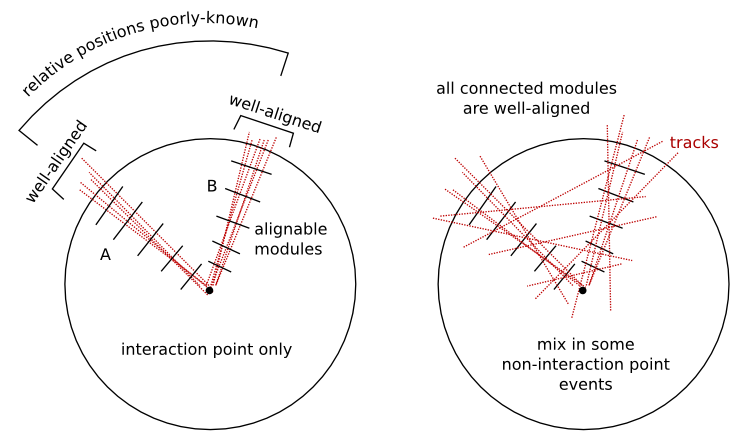
\includegraphics[width=0.7\linewidth]{why_non-collisions_are_important.png}
\end{center}

\item Alignment technical triggers guarantee that we will get cosmics
  and beam-halo, even during high-luminosity collisions runs

\item However, this year we will have a lot of non-collisions data runs with
  wide-open triggers
\end{itemize}
%% \hspace{-0.83 cm} \textcolor{darkblue}{\Large Outline2}
\end{frame}

\begin{frame}
\frametitle{History}
\small

\begin{itemize}\setlength{\itemsep}{0.25 cm}
\item 2\_0\_0 release deadline: I couldn't find anyone to implement these HLT paths, so I did it because it didn't look too hard
\item Release validation is a long-term commitment--- we needed to find people who can dedicate the time
\begin{itemize}\setlength{\itemsep}{0.25 cm}
\item CSC beam-halo trigger: Joe Gartner (wrote L1 emulator, doing physics studies with beam-halo events)
\item tracker beam-halo BSC: no one formally assigned, though Andrea Parenti is doing tracker alignment studies with beam-halo
\item tracker cosmic rays: no one formally assigned, though Jean-Roch Vlimant has done some work on the tracker cosmics trigger paths
\end{itemize}
\item Search for manpower has been raised many times in tracker DPG (more detail on subsequent slides)
\end{itemize}
\end{frame}

\begin{frame}
\frametitle{CSC beam-halo triggers}
\small
Actively studied in both data and Monte Carlo by Joe Gartner,

but not yet formalized into a validation suite

\begin{columns}
\column{0.5\linewidth}
\begin{itemize}
\item focused on commissioning real L1 trigger in CRUZET
\item informally verified stable releases: 1\_8\_0, 2\_0\_7, and {\bf 2\_0\_11} (these plots)
\item true validation suite soon
\end{itemize}

\vspace{0.3 cm}

\column{0.5\linewidth}
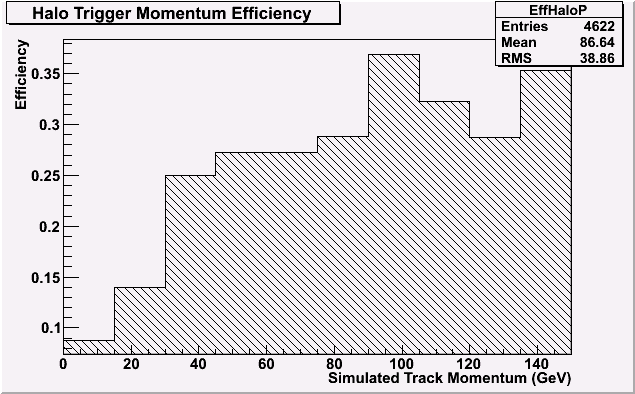
\includegraphics[width=\linewidth]{HaloTriggerMomentum.png}
\end{columns}

\begin{columns}
\column{0.5\linewidth}
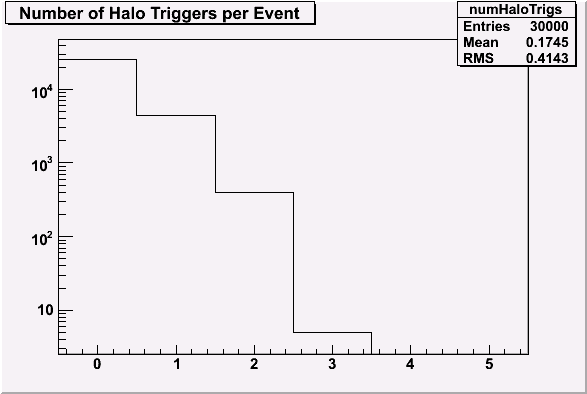
\includegraphics[width=\linewidth]{NumHaloTrigs.png}
\column{0.5\linewidth}
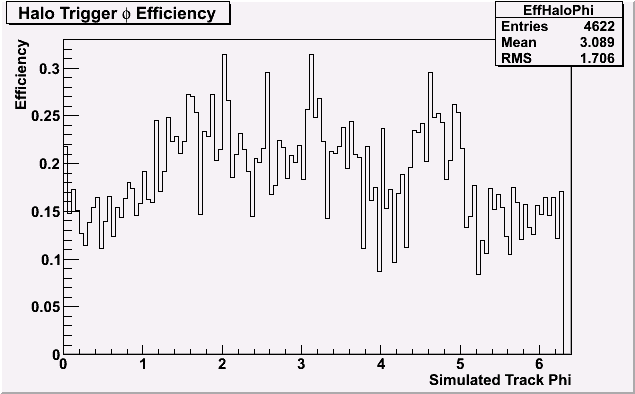
\includegraphics[width=\linewidth]{PhiEfficiency.png}
\end{columns}
\end{frame}

\begin{frame}
\frametitle{Tracker beam-halo BSC}
\small

\hspace{-0.83 cm} \textcolor{darkblue}{\Large (Context:} might be necessary even for dedicated beam-halo runs{\Large )}

\vfill
\begin{itemize}\setlength{\itemsep}{0.25 cm}
\item Andrea Parenti is not formally responsible for the validation suite, but his work is the most related

\item Until recently, validation work could not begin because L1 emulator did not exist

\item L1 emulator added by Muriel: tested in MinBias, but not successfully in beam-halo sample

\item Urgency for someone to take on this task has escalated since it
  is now possible to generate triggered events in MC and time is getting short for beam-halo data
\end{itemize}
\end{frame}

\begin{frame}
\frametitle{Tracker cosmic rays}
\small

\begin{itemize}\setlength{\itemsep}{0.35 cm}
\item Jean-Roch Vlimant is not formally responsible for the validation suite, but his work is the most related

\item He has developed more advanced HLT paths; these may supercede the original HLT\_TrackerCosmics

\item L1 RPC technical trigger emulator code exists, but has never been published in a release

\item Jean-Roch has been working on instead getting the L1 bit from a DT trigger which requires the track to point into the tracker

\item His HLT paths do track-finding, require unpacking of tracker
  hits, may be too time-expensive to be used in collisions runs unless
  L1 is very selective

\end{itemize}
\end{frame}

%% \section*{First section}
%% \begin{frame}
%% \begin{center}
%% \Huge \textcolor{blue}{First section}
%% \end{center}
%% \end{frame}

\begin{frame}
\frametitle{Conclusions}
\small

\begin{itemize}\setlength{\itemsep}{0.1 cm}

\item Triggers for non-collisions events will be {\it more} necessary
  at high luminosity when we don't have dedicated non-collisions runs,
  but it is worthwhile getting them to work now

\item CSC beam-halo path is well-covered, but until now focus hasn't
  been on software validation

\item L1 emulator for tracker triggers was in a less advanced state,
  but that has changed recently

\item Tracker cosmic ray triggers may be reorganized soon;
  HLT\_TrackerCosmics might be replaced

\item (Also studying Mika Huhtinen's pixel MinBias trigger for tracker\ldots)

\item Tracker DPG still needs to find people to maintain trigger
  validation in the long-term

\item In no sense have these paths been forgotten about!  We know
  software validation is important, but the people involved are
  stretched thin by other DPG tasks, some of which is closely related.
\end{itemize}
\label{numpages}
\end{frame}

\end{document}
